%\title{Исследование производственных систем с маршрутизацией, зависящей от состояния}
%\author{Салин Роман Владимирович}
%\institute{САРАТОВСКИЙ ГОСУДАРСТВЕННЫЙ УНИВЕРСИТЕТ ИМЕНИ Н.Г. ЧЕРНЫШЕВСКОГО}
%\date{Саратов, 2014}

\begin{frame}[plain]
\begin{center}
Министерство образования и науки Российской Федерации\\
САРАТОВСКИЙ ГОСУДАРСТВЕННЫЙ УНИВЕРСИТЕТ\\
ИМЕНИ Н. Г. ЧЕРНЫШЕВСКОГО
\end{center}

%\vspace{0.5cm}
%\begin{flushright}
%\parbox{6.8cm}{
%\raggedright
%  Кафедра системного анализа \\ и автоматического управления
%}
%\end{flushright}

\vfill

\begin{center}
\textbf{Исследование производственных систем с маршрутизацией,\\зависящей от состояния}\\
\medskip
ВЫПУСКНАЯ КВАЛИФИКАЦИОННАЯ РАБОТА СПЕЦИАЛИСТА
\end{center}
\begin{flushleft}
студента 5 курса 511 группы\\
специальности 010501 --- прикладная математика и информатика\\
факультета компьютерных наук и информационных технологий\\
Салина Романа Владимировича
\end{flushleft}

\vfill

\noindent
\begin{flushleft}
Научный руководитель\\
доцент, к.ф.-м.н. \hfill В. И. Долгов\\
\end{flushleft}

\vfill

\begin{center}
Саратов 2014
\end{center}
\end{frame}

% ------------------------------------------------------------------- %

\begin{frame} \frametitle{Цели и задачи работы}
\begin{itemize}
\item исследование производственных систем с маршрутизацией, зависящей от состояния;
\item разработка алгоритма метода анализа производственных систем с маршрутизацией, зависящей от состояния;
\item программная реализация алгоритма;
\item проведение численных экспериментов с разработанной программой.
\end{itemize}
\end{frame}

% ------------------------------------------------------------------- %

\begin{frame} \frametitle{Гибкие производственные системы}
\begin{itemize}
\item $\mathscr{C}=\{C_i\}$ --- множество рабочих станций ГПС, $i \in I \equiv \{ i ~|~ i=1,...,L \}$; $I_t \subseteq I$;

\item $\mathscr{T}=\{1,2,...,T\}$ --- множество типов деталей ГПС;

\item $\kappa_i$ --- число параллельно работающих приборов на станции $C_i$, $i=1,...,L$; $\kappa = (\kappa_i)$;

\item $C_0$ --- система транспортировки; $\kappa_0$~--- число транспортеров;

\item $N_t$ --- число деталей типа $t$ в ГПС, $\sum\limits_t N_t = N$; $\mathbf{N}=(N_t)$, $t=1,...,T$;

\item $s_{it}$ --- емкость рабочей станции $C_i$ для деталей типа $t$, $i \in I_t$, $t=1,...,T$; $s = (s_{it})$;

\item $\mu_{it}$ --- интенсивность обработки детали типа $t$ на станции $C_i$, $i \in I_t$, $t=1,...,T$;

\item $D_i = RANDOM$ --- дисциплина обработки на станциях $C_i,~i=1,...,L$.

\item $\overline{\eta} = (\overline{\eta}_0, \overline{\eta}_1,...,\overline{\eta}_L)$ --- состояние ГПС, где $\overline{\eta}_i = (n_{i1},...,n_{iT})$~--- состояние рабочей станции $C_i$, $i=1,...,L$.
\end{itemize}
\end{frame}

% ------------------------------------------------------------------- %

\begin{frame} \frametitle{Гибкие производственные системы}
\begin{figure}[H]
  \centering
  \includegraphics[width=0.9\textwidth]{fms}
  \label{fig:main}
\end{figure}
\end{frame}

% ------------------------------------------------------------------- %

\begin{frame} \frametitle{Маршрутизация}
В производственной системе имеет место вероятностная маршрутизация в кратчайшую очередь:
\vfill
\begin{equation}
 \theta_{0t,it} = \frac{r_{it}(n_{it})} {r_{0t}(n_{0t})},
\label{eq:2.2}
\end{equation}
\vfill
где $r_{it}(\cdot)$ и $r_{0t}(\cdot)$~--- две линейные функции:
\vfill
\begin{equation*}
 r_{it}(n_{it}) = s_{it} - n_{it} ~ \text{и} ~ r_{0t}(n_{0t}) = \sum_{C_i \in I_t} s_{it} + n_{0t} - N_t,
\end{equation*}
$i=1,...,L$, $t=1,...,T$.
\vfill
\end{frame}

% ------------------------------------------------------------------- %

\begin{frame} \frametitle{Стационарное решение}
\textbf{Теорема\footnotemark.} Марковский процесс $\overline{\eta}(\tau)$, определенный в пространстве состояний $S$ и управляемый PSQ--маршрутизацией, как определено в~(\ref{eq:2.2}), является обратимым относительно времени и имеет следующую мультипликативную форму стационарного распределения вероятностей:
 \begin{equation}
  \pi(\overline{\eta}) = G^{-1} \prod_{i=0}^L \left[ \prod_{j=1}^{n_i} \nu_i^{-1} (j) \right]
  \left[ \prod_{t=1}^T \prod_{j=1}^{n_{it}} \frac{r_{it} (j - 1 + \delta_{i0})}{j\mu_{it}} \right], \quad \overline{\eta} \in S ,
  \label{eq:2.4}
 \end{equation}
где $\delta_{i0}=1$, если $i=0$, иначе $\delta_{i0}=0$, $G$~--- нормализующая константа и
\begin{equation*}
\nu_i(n_i) = \frac{\min(n_i, \kappa_i)}{n_i} .
\end{equation*}
\footnotetext[1]{Yao D. D., Buzacott J. A. Modeling a class of state-dependent routing in flexible manufacturing systems~// Annals of Operations Research.~-- 1985.~-- No. 3.~-- P. 153-167.}
\end{frame}

% ------------------------------------------------------------------- %

\begin{frame} \frametitle{Структура алгоритма}
\textbf{Шаг 1. Ввод исходных данных}

\begin{itemize}
\item $L$~--- число СМО в СеМО;
\item $\mathbf{N}=(N_t)$~--- вектор начального числа требований в СеМО, $t=1,...,T$;
\item $\kappa=(\kappa_i)$~--- вектор числа приборов в системах обслуживания СеМО, $i=0,...,L$;
\item $s=(s_{it})$~--- матрица емкостей систем в СеМО, $i=0,...,L,~t=1,...,T$;
\item $\mu=(\mu_{it})$~--- матрица интенсивностей обслуживания требований системами СеМО, $i=0,...,L,~t=1,...,T$.
\end{itemize}

\textbf{Шаг 2.} Положить $i = 1$.

\textbf{Шаг 3. Перестановка СМО $\boldsymbol{C_i}$ и $\boldsymbol{C_L}$}

\end{frame}

% ------------------------------------------------------------------- %

\begin{frame} \frametitle{Структура алгоритма}

\textbf{Шаг 4. Вычисление стационарного распределения вероятностей состояний СМО $\boldsymbol{C_i}$}

\emph{Входные данные:} $L$, $T$, $\mathbf{N}=(N_t)$, $\kappa=(\kappa_i)$, $s=(s_{it})$, $\mu=(\mu_{it})$, $i=0,...,L,~t=1,...,T$.\\
\emph{Выходные данные:} $\pi_i(\mathbf{n},\mathbf{N})$, $i=1,...,L$.

\textbf{Шаг 5. Обратная перестановка СМО $\boldsymbol{C_L}$ и $\boldsymbol{C_i}$}

\textbf{Шаг 6.} Если $i < L$, то положить $i=i+1$ и перейти на \textbf{шаг 3}, иначе перейти к \textbf{шагу 7}.

\textbf{Шаг 7. Вычисление стационарных характеристик СеМО}

\textbf{Шаг 8. Вывод результатов}

\begin{itemize}
\item $\overline{n}_{it}$~--- м. о. числа требований, $i=0,...,L,~t=1,...,T$;
\item $\lambda_{it}$~--- интенсивности потока требований, $i=0,...,L,~t=1,...,T$;
\item $\psi_{it}$~--- коэффициенты использования обслуживающих приборов, $i=0,...,L,~t=1,...,T$.
\end{itemize}
\end{frame}

% ------------------------------------------------------------------- %

\begin{frame} \frametitle{Интерфейс программы}
\begin{figure}[H]
  \centering
  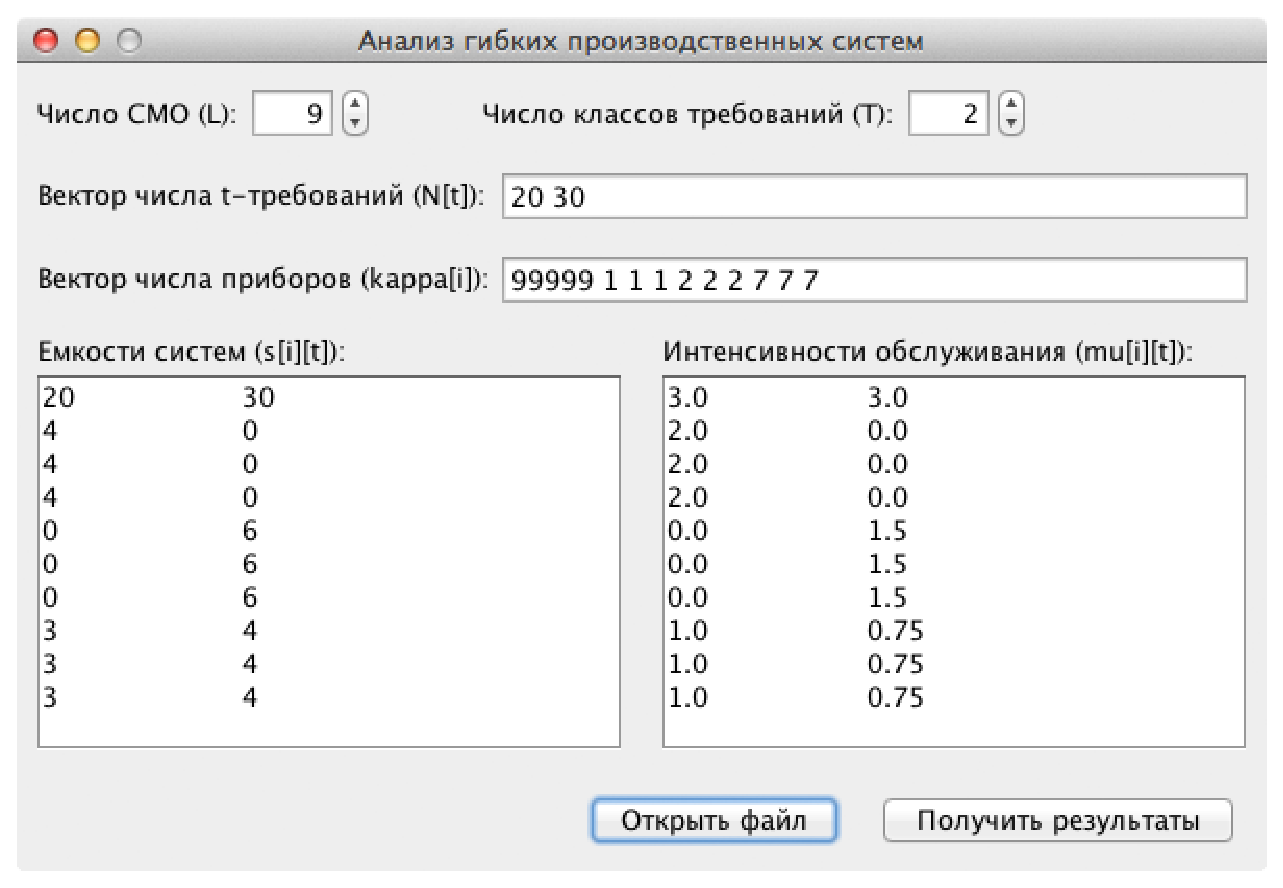
\includegraphics[width=0.9\textwidth]{main}
  \label{fig:main}
\end{figure}
\end{frame}

% ------------------------------------------------------------------- %

\begin{frame} \frametitle{Интерфейс программы}
\begin{figure}[H]
  \centering
  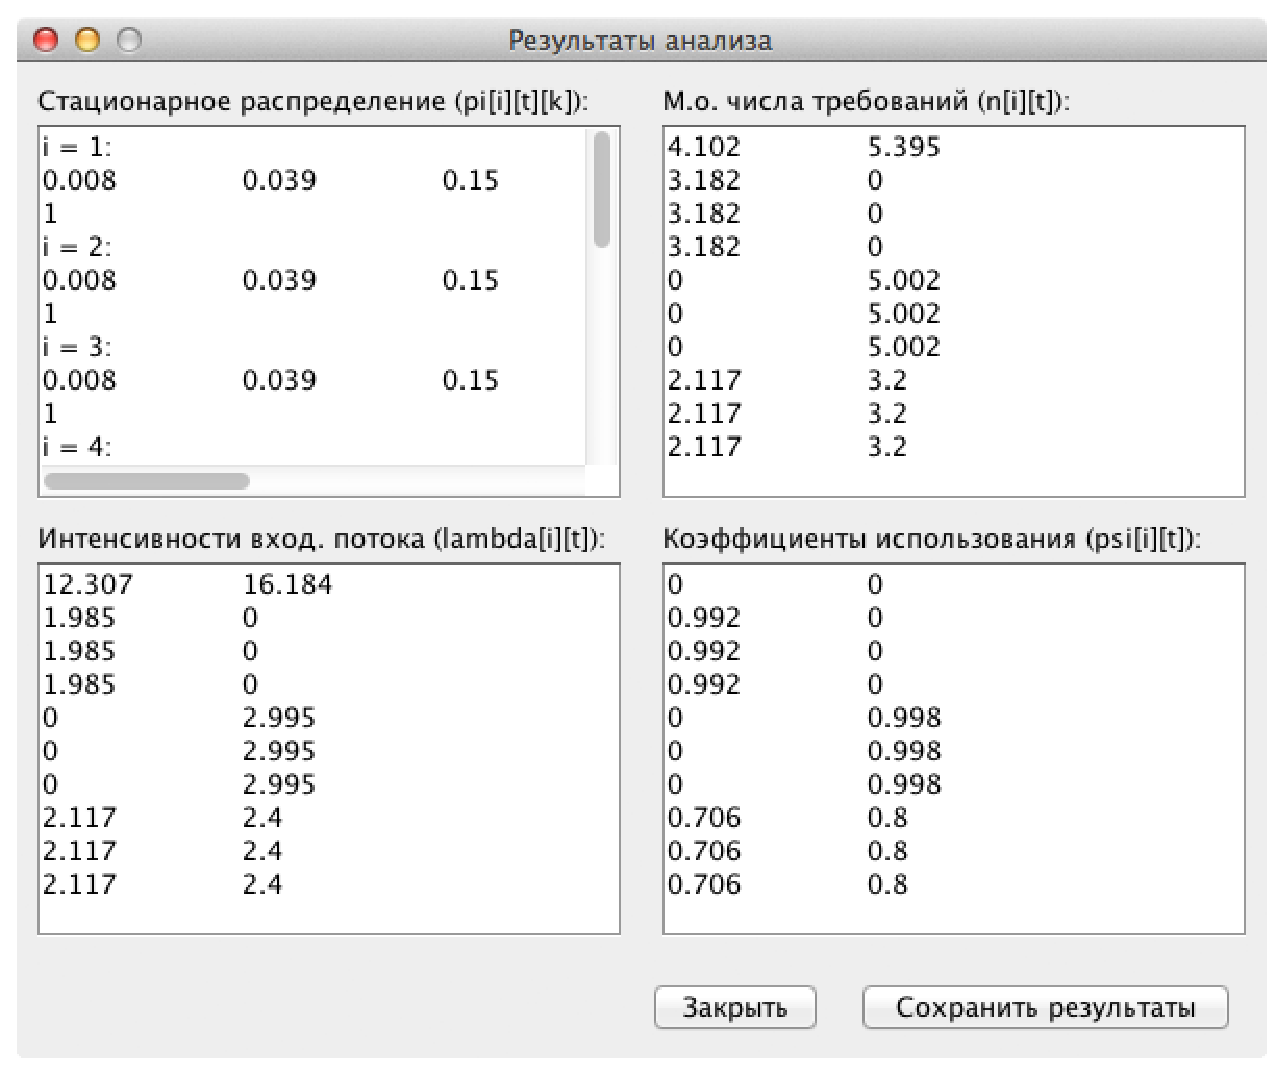
\includegraphics[width=0.8\textwidth]{results}
  \label{fig:main}
\end{figure}
\end{frame}

% ------------------------------------------------------------------- %

\begin{frame} \frametitle{Пример}
$L=9$; $T=2$; $\mathbf{N}=(20,30)$; \\
$I_1=\{1,2,3,7,8,9\}$, $I_2=\{4,5,6,7,8,9\}$; \\
$\kappa_1=\kappa_2=\kappa_3=1$; $\kappa_4=\kappa_5=\kappa_6=2$; $\kappa_7=\kappa_8=\kappa_9=7$; \\
$\mu_{11}=\mu_{21}=\mu_{31}=2$; $\mu_{42}=\mu_{52}=\mu_{62}=1,5$; $\mu_{71}=\mu_{81}=\mu_{91}=1$; $\mu_{72}=\mu_{82}=\mu_{92}=0,75$; \\
$s_{11}=s_{21}=s_{31}=4$; $s_{42}=s_{52}=s_{62}=6$; $s_{71}=s_{81}=s_{91}=3$; $s_{72}=s_{82}=s_{92}=4$. \\
Для $C_0$: $\mu_{01}=\mu_{02}=3$; $s_{01}=20$; $s_{02}=30$. \\

{\renewcommand{\arraystretch}{1.5}%
\begin{table}[H]
\begin{tabular}{|c|c|c|c|c|c|c|}
\hline
$C_i$  &  \multicolumn{2}{c|}{$C_0$}  &  $C_{1, 2, 3}$  &  $C_{4, 5, 6}$  &  \multicolumn{2}{c|}{$C_{7, 8, 9}$} \cr
\hline
$t$ &  Тип 1  &  Тип 2  &  Тип 1  &  Тип 2  &  Тип 1  &  Тип 2 \cr
\hline
$\overline{n}_i$  &  4,102  &  5,395  &  3,182  &  5,002  &  2,117  &  3,200 \cr
\hline
$\lambda_i$  & 12,307  & 16,184  &  1,985  &  2,995  &  2,117  &  2,400 \cr
\hline
$\psi_i$  &    --    &    --    &  0,993  &  0,998  &  0,706  &  0,800 \cr
\hline
\end{tabular}
\end{table}}
\end{frame}

% ------------------------------------------------------------------- %

\begin{frame} \frametitle{Результаты работы}
\begin{itemize}
\item рассмотрены производственные системы с маршрутизацией, зависящей от состояния;
\item разработан алгоритм метода анализа производственных систем с маршрутизацией, зависящей от состояния;
\item разработана программа, вычисляющая основные стационарные характеристики производственных систем с маршрутизацией, зависящей от состояния;
\item проведены численные эксперименты с разработанной программой и приведены соответствующие результаты.
\end{itemize}
\end{frame}
